\documentclass[10pt]{article}  

%%%%%%%% PREÁMBULO %%%%%%%%%%%%
\usepackage[english]{babel} %Indica que escribiermos en español
\usepackage[utf8]{inputenc} %Indica qué codificación se está usando ISO-8859-1(latin1)  o utf8  
\usepackage{amsmath} % Comandos extras para matemáticas (cajas para ecuaciones,
% etc)
\usepackage{amssymb} % Simbolos matematicos (por lo tanto)
\usepackage{graphicx} % Incluir imágenes en LaTeX
\usepackage{color} % Para colorear texto
\usepackage{subfigure} % subfiguras
\usepackage{ulem}
\usepackage{amsmath}%%Usar ecuaciones
%%%%%%%%%%%%%CODIGO%%%%%%%%%%%%%%%%%%%%%%
\usepackage{listings} %Sirve para pegar codigo fuente de programas
\usepackage{caption}
\DeclareCaptionFont{white}{\color{white}}
\DeclareCaptionFormat{listing}{%
  \parbox{\textwidth}{\colorbox{gray}{\parbox{\textwidth}{#1#2#3}}\vskip-4pt}}
\captionsetup[lstlisting]{format=listing,labelfont=white,textfont=white}
\lstset{frame=ltrb,xleftmargin=\fboxsep,xrightmargin=-\fboxsep}
%%%%%%%%%%%%%CODIGO%%%%%%%%%%%%%%%%%%%%%%
\usepackage{float} %Podemos usar el especificador [H] en las figuras para que se
% queden donde queramos
\usepackage{capt-of} % Permite usar etiquetas fuera de elementos flotantes
% (etiquetas de figuras)
\usepackage{enumerate} % enumerados
\usepackage{sidecap} % Para poner el texto de las imágenes al lado
	\sidecaptionvpos{figure}{c} % Para que el texto se alinie al centro vertical
\usepackage{caption} % Para poder quitar numeracion de figuras
\usepackage{commath} % funcionalidades extras para diferenciales, integrales,
% etc (\od, \dif, etc)
\usepackage{cancel} % para cancelar expresiones (\cancelto{0}{x})
 
\usepackage{anysize} 					% Para personalizar el ancho de  los márgenes
\marginsize{2cm}{2cm}{2cm}{2cm} % Izquierda, derecha, arriba, abajo

\usepackage{appendix}

%Para la creación de tablas
\usepackage{array}
\newcolumntype{P}[1]{>{\centering\arraybackslash}p{#1}}
\newcolumntype{M}[1]{>{\centering\arraybackslash}m{#1}}
\usepackage{makecell}



%Para la creacion de cuadros de colores
\usepackage{tcolorbox}
\tcbuselibrary{listingsutf8}
% Cuadro numerado para ejemplos de cuadros de colores
\newtcolorbox[auto counter, number within=section]{example}[2][]
{colback=red!5!white,colframe=red!75!black,
fonttitle=\bfseries, title=Example~\thetcbcounter: #2,#1}

\newtcolorbox[auto counter, number within=section]{tip}[2][]
{colback=green!5!white,colframe=green!75!black,
fonttitle=\bfseries, title=Tip~\thetcbcounter: #2,#1}

% Para que las referencias sean hipervínculos a las figuras o ecuaciones y
% aparezcan en color
\usepackage[colorlinks=true,plainpages=true,citecolor=blue,linkcolor=blue]{hyperref}
%\usepackage{hyperref} 
% Para agregar encabezado y pie de página
\usepackage{fancyhdr} 
\pagestyle{fancy}
\fancyhf{}
\fancyhead[L]{\footnotesize VPLWVST} %encabezado izquierda
\fancyhead[R]{\footnotesize VP-TB}   % dereecha
\fancyfoot[R]{\footnotesize Tutorial A}  % Pie derecha
\fancyfoot[C]{\thepage}  % centro
\fancyfoot[L]{\footnotesize VisualPro: A Lightweight; Visual Scripting Tool}  %izquierda
\renewcommand{\footrulewidth}{0.4pt}


\usepackage{listings} % Para usar código fuente
\definecolor{dkgreen}{rgb}{0,0.6,0} % Definimos colores para usar en el código
\definecolor{gray}{rgb}{0.5,0.5,0.5} 
% configuración para el lenguaje que queramos utilizar
\lstset{basicstyle=\ttfamily,
   basicstyle=\ttfamily,
   keywordstyle=\color{blue},
   commentstyle=\color{red},
   stringstyle=\color{dkgreen},
   numberstyle=\tiny\color{gray},
   stepnumber=1,
   numbersep=10pt,
   backgroundcolor=\color{white},
   tabsize=4,
   showspaces=false,
   breaklines=true,
   showstringspaces=false}

\newcommand{\sen}{\operatorname{\sen}}	% Definimos el comando \sen para el seno
%en español
%%%%%%%% TERMINA PREÁMBULO %%%%%%%%%%%%

\begin{document}

%%%%%%%%%%%%%%%%%%%%%%%%%%%%%%%%%% PORTADA %%%%%%%%%%%%%%%%%%%%%%%%%%%%%%%%%%%%%%%%%%%%
																					%%%
\begin{center}																		%%%
\newcommand{\HRule}{\rule{\linewidth}{0.5mm}}									%%%\left
 																					%%%
\begin{minipage}{0.48\textwidth} \begin{flushleft}

\includegraphics[scale = 0.15]{Figures/Logo/UWTSD-Logo}
\end{flushleft}\end{minipage}
\begin{minipage}{0.48\textwidth} \begin{flushright}

\includegraphics[scale = 0.4]{Figures/Logo/VP-Logo-Large}
\end{flushright}\end{minipage}

													 								%%%
\vspace*{-1.5cm}								%%%
																					%%%	
\textsc{\huge Visual Pro\\ \vspace{5px} Tutorial B}\\[1.5cm]	

\textsc{\LARGE A beginners guide to Visual Scripting}\\[1.5cm]													%%%

\textsc{\Large VisualPro: A Lightweight; Visual Scripting Tool}\\[0.5cm]

    																				%%%
 			\vspace*{1cm}																		%%%
																					%%%
\HRule \\[0.4cm]																	%%%
{ \huge \bfseries Tutorial: Functions and Variables}\\[0.4cm]	%%%
 																					%%%
\HRule \\[1.5cm]																	%%%
 																				%%%
																					%%%
\begin{minipage}{0.4\textwidth}													%%%
\begin{flushleft} \large															
\textit{Authors:}\\
Edward Patch\\
Student Number: 1801492\\
\end{flushleft}																		%%%
\end{minipage}		
																%%%
\begin{minipage}{0.5\textwidth}		
\vspace{-0.6cm}											%%%
\begin{flushright} \large															%%%
\textit{Supervisor:} \\
Mike Dacey														%%%									
\end{flushright}																	%%%
\end{minipage}	
\vspace*{1cm}

\vspace{2cm} 																				
\begin{center}																					
{\large 16 February 2022}																	%%%
 			\end{center}												  						
\end{center}							 											
																					
\newpage																		
%%%%%%%%%%%%%%%%%%%% TERMINA PORTADA %%%%%%%%%%%%%%%%%%%%%%%%%%%%%%%%

\tableofcontents
\thispagestyle{fancy}

\newpage
\section{Learning Objectives}
The following learning objectives are as follows:
\begin{enumerate}
    \item To declare functions in a Functional Programming (FP) style rather than an OOP style.
    \item To declare variables in both global scope \textbf{(considered bad practice)} and function scope.
\end{enumerate}


\newpage
\section{Introduction}
  Focus on the FP style, which gives the chance to increase existing skill level to explore both OOP and FP style languages. Supported languages in VisualPro are C and C++.

  \begin{tip}{Fun Fact:}
    C++ is an extension of C that offers both FP and OOP style language, making the language a powerful language.
  \end{tip}

  \subsection{What is the Differences?}
    OOP style enables the creation of objects, whereas FP style contains functional structure. However, C does allow the creation of a `struct' that is similar to a class, however, it only allows variables. It is great for creating reusable data structures but do not Constructors or Deconstructors that play a big part in memory management.
    
    An example of C\# (OOP Style) vs. C (FP Style):
    \begin{example}{OOP Style}
      \begin{lstlisting}[language=java]
        using System; // Provides the Console.WriteLine function from the `System' library.

        class Program { 
          static void Main(string[] args) {
            int x = 6, y = 45;
            Console.WriteLine("x + y = " + (x * y).ToString()); 
            // result: 270 (The ToString method converts the x * y calculation to a string and appends to the string).
          }
        }
      \end{lstlisting}
    \end{example}

    \begin{example}{FP Style}
      \begin{lstlisting}[language=c]
        #include <stdio.h> /* Provides the printf function from the 
        `stdio' library. */

        int main(int argc, char** argv) {
            int x = 6, y = 45;
            printf("x + y = %i", x * y); // result: 270 (%i means first parameter is an integer and includes it to the string).
            
            return 0;
        }
      \end{lstlisting}
    \end{example}

    Note that the OOP style relies on encapsulation, whereas the C language or any other language is FP.

\newpage
\section{VisualPro Environment}
\label{sec:vp-env}
    \subsection{Features}
        VisualPro offers a few features such as:
        \begin{itemize}
            \item Classes, Functions and Arguments, and Variables.
            \item Saving in Multiple Languages.
            \item Drag and Drop Elements and Text Areas.
            \item Property Windows to Control Arguments and Relationships.
        \end{itemize}

    \subsection{Known Bugs}
        A couple of bugs include:-
        \begin{itemize}
            \item Arguments for functions are not currently available.
            \item Deleting containers does not mathematically reset the following location or move existing containers backwards.
        \end{itemize}

    \subsection{Saving Progress}
        After completing a tutorial, select the language and press save.

        \begin{tip}{Compatibility}
            As mentioned previously, not all languages support object-orientation. If a language is not compatible with a particular keyword, the code generator will ignore the selected syntax object.

            \textbf{Example Language:} C is not supported.
        \end{tip}

\newpage
\section{Terminology}
\label{sec:terminology}
    \subsection{What is a function?}
      Like a method, a function exists in the global scope of an FP style language, such as the C language. A function can return data like an integer or a string or a `void' data type that returns nothing. It is also important to note that arguments are the function's inputs that enable data to pass through the function scope.

      Three examples of different functions and their purposes:
      \begin{example}{Function: \textbf{VOID} Return Type}
        \begin{lstlisting}[language=c]
          #include <stdio.h>

          // The function returns nothing.
          // The function accepts no arguments.
          void PrintHelloWorld()
          { printf("Hello World"); }

          int main(int argc, char** argv)
          {
            // The call to the function.
            PrintHelloWorld();
            return 0;
          }
        \end{lstlisting}
      \end{example}

      \begin{example}{Function: \textbf{VOID} Return Type | \textbf{Integer} Argument}
        \begin{lstlisting}[language=c]
          #include <stdio.h>

          // The function returns nothing.
          // The function accepts one argument (integer).
          void PrintX4(int x)
          { printf("%i * 4 = %i", x, x*4); }

          int main(int argc, char** argv)
          {
            PrintX4(10); // Result: 10 * 4 = 40
            return 0;
          }
        \end{lstlisting}
      \end{example}

      \begin{example}{Function: \textbf{Integer} Return Type | \textbf{Integer} Argument}
        \begin{lstlisting}[language=c]
          #include <stdio.h>

          // The function returns an integer.
          // The function accepts two arguments (integer and integer).
          int PrintXY(int x, int y)
          { return x * y; }

          int main(int argc, char** argv)
          {
            int x = PrintXY(2, 7);
            printf("2 * 7 = %i", x); // result: 2 * 7 = 14

            return 0;
          }
        \end{lstlisting}
      \end{example}

\newpage
\section{Functional Structure}
\label{sec:functional-structure}
    \subsection{Exercise: Understanding the Basics}
      A function exists outside of a class and within the global scope. When declaring and defining a function, the location of the declaration must be above the definition of the function.
      
      A couple of examples are on display below:

      \begin{example}{Declaration of a Function (A):}
        \begin{lstlisting}[language=c]
          #include <stdio.h>

          // Declaration and Definition
          float XMultiplyY(double x, double y) {
              return x * y;
          }

          int main(int argc, char** argv) {
            printf("8.87 * 2.65 = %f", XMultiplyY(8.87, 2.65)); 
            // result: 23.505501
            return 0;
          }
        \end{lstlisting}
      \end{example}

      Alternatively, defining a function is to declare above the `main' function and defining the function below the `main` function. For example:

      \begin{example}{Declaration of a Function (B):}
        \begin{lstlisting}[language=c]
          #include <stdio.h>

          // Declaration
          float XMultiplyY(double x, double y);

          int main(int argc, char** argv) {
            printf("8.87 * 2.65 = %f", XMultiplyY(8.87, 2.65)); 
            // result: 23.505501
            return 0;
          }

          // Definition
          float XMultiplyY(double x, double y) {
              return x * y;
          }
        \end{lstlisting}

        Also, the declaration could belong to a header file, including the definition with the header tag.
      \end{example}

      \begin{tip}{Evidencing}
        \textbf{Necessary:} Make sure to copy each exercise code to the survey when asked. A reference of the survey question helps find the corresponding survey question to paste the final code.
      \end{tip}

    \subsection{Exercise: Toaster Functionality}
      A toaster has three primary functions, heat up, cool down and timer. First, let us drag a function onto the Work Area panel within VisualPro. Name this function, `HeatUp'. A functional structure does not have Access Modifiers, so leave this field blank. Now, set the return value (datatype) as void. Drag another function onto the Work Area panel, naming the function `CoolDown' and set the return value as void. Finally, drag the last function onto the Work Area panel, naming the function `Timer' and set the return value as bool (for Boolean (true/false)).

      \textbf{Make sure to save the file in the C language and upload the file's contents to the relevant section of the survey.} 

      \textbf{Did it look like this visually?}
        \begin{figure}[h]
          \centering
          {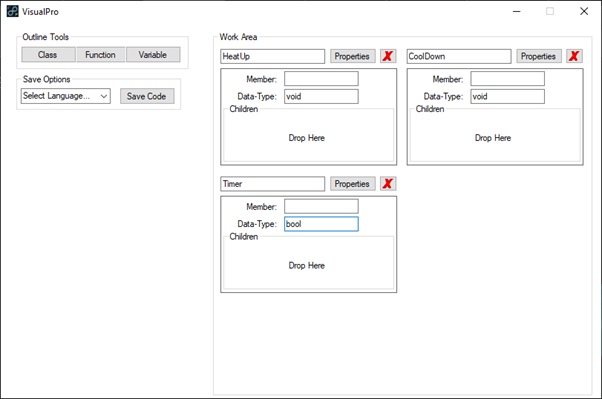
\includegraphics[scale=0.75]{Figures/Exercises/TutB-SecA-1.png}}
          \caption{VisualPro - Exercise A}
          \label{fig:vp-eA}
        \end{figure}

      \textbf{Expected Code Generation:-}\\
        This code should look similar to this:
        \begin{example}{Toaster Functionality}
          \begin{lstlisting}
            void HeatUp()
            {

            }

            void CoolDown()
            {

            }

            bool Timer()
            {

            }
          \end{lstlisting}
        \end{example}

    \subsection{Excercise: Toaster Variables}
        When thinking about a toaster, think of a few variables. There is no right or wrong answer to this question. Create the variables on a blank VisualPro pad, by dragging and dropping the variables on the Work Area panel. Again, there is no need for a member.

        \textbf{Note:} This way, the variables are within the global scope and is not good practice. \textbf{Make sure to save the file in the C language and upload the file's contents to the relevant section of the survey.}

        \textbf{Did it look like this visually?}
          \begin{figure}[h]
            \centering
            {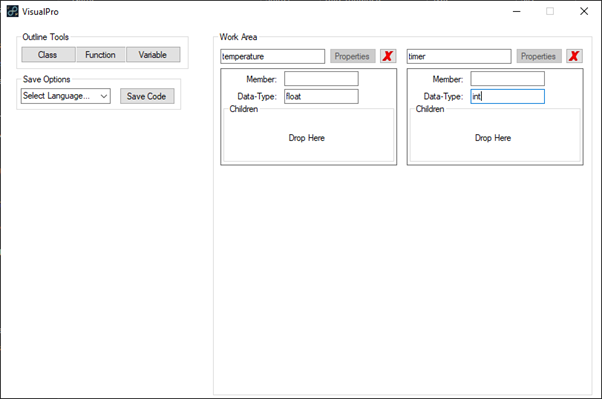
\includegraphics[scale=0.75]{Figures/Exercises/TutB-SecB-1.png}}
            \caption{VisualPro - Exercise B}
            \label{fig:vp-eB}
          \end{figure}

        \textbf{Expected Code Generation:-}\\
          \begin{example}{Toaster Variables}
            \begin{lstlisting}[language=c]
              float temperature;
              int timer;
            \end{lstlisting}
          \end{example}
    \subsection{Excercise: Functions and Variables}

    \subsection{Exercise: Try It Yourself (TIY)}

\section{Keywords}
\label{sec:keywords}
    \begin{itemize}
      \item FP - Functional Programming.
      \item OOP - Object-Oriented Programming.
    \end{itemize}

%%%%%%% References %%%%%%%%
\clearpage
\nocite{*}
\small{\bibliographystyle{IEEEtran}
\bibliography{ref}}
%%%%%%% References %%%%%%%%      
\end{document}